\section{深度学习}\label{sec:nn-dl}

\subsection{前向传播}

设有训练样本为$\mathbf{X}$,其经过特征提取后共有$m$个特征,则对于任意样本,有$\mathbf{X} \in \mathbb{R}^{m}$,通常样本向量为列向量,行数即为其特征维度的大小。神经网络结构,如图\ref{fig:nn}所示,对于多层神经网络,其包含输入层、隐藏层、输出层。
\begin{figure}[hbp]
  \centering
  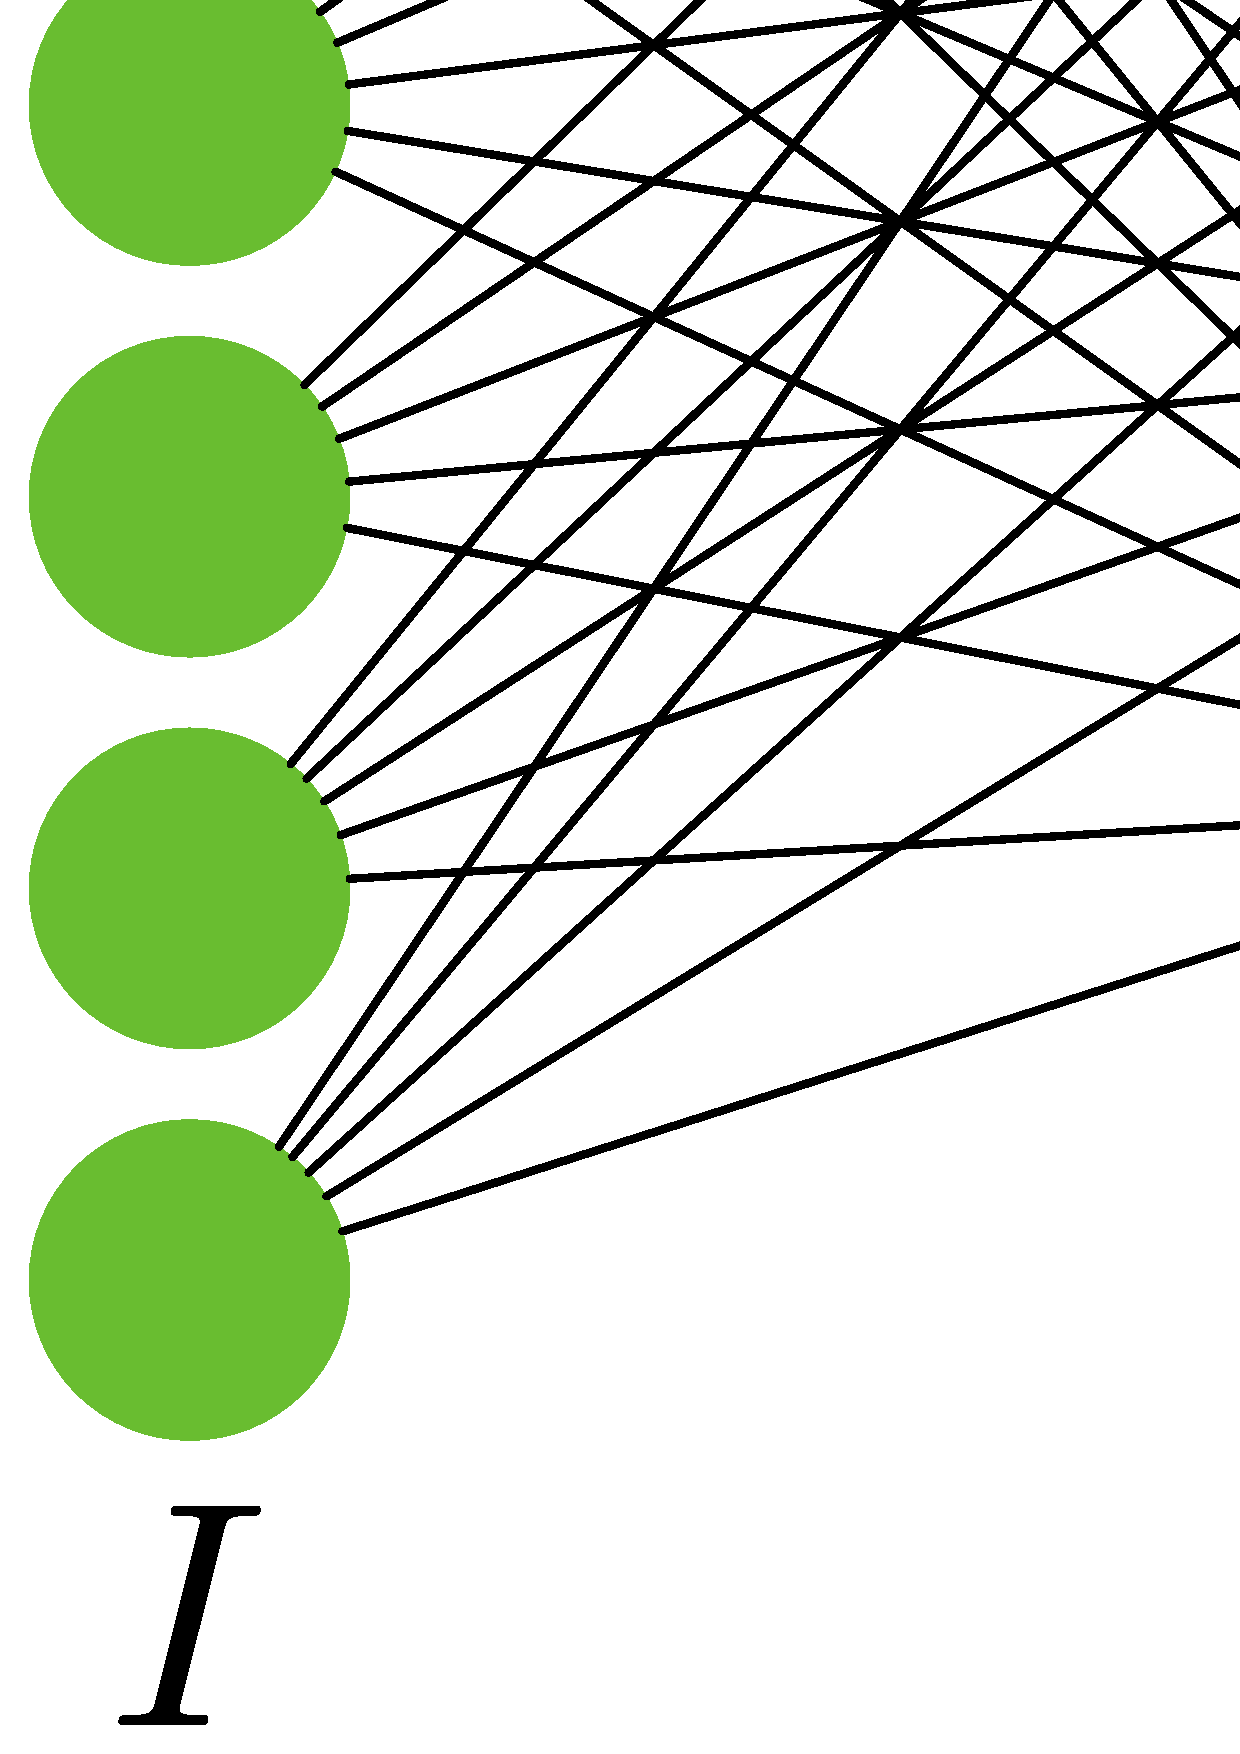
\includegraphics[width=.7\textwidth]{figures/nn.pdf}
  \caption{神经网络示意图}
  \label{fig:nn}
\end{figure}

神经网络通过前向传播得出模型的预测结果,即对结果的拟合。其过程如下,对于输入$\mathbf{X}$,其输入到第一层隐藏层,进行线性激活:$\mathbf{Z}^{[1]} = \mathbf{W}^{[1]} \times \mathbf{X} + b^{[1]}$,由于多次线性变换的结果仍未线性变换,则需要在线性激活函数后加入非线性函数再次激活。则对于第1层隐藏层,其激活后的输出结果为$\mathbf{A}^{[1]}=\sigma (\mathbf{Z}^{[1]})$,其中$\sigma$为激活函数。

对于从第$l$层隐藏层到第$l+1$层隐藏层,则$l+1$层输入为$l$层的激活后输出$\mathbf{A}^{[l]}$,则前向传播过程为:
\begin{equation}
  \mathbf{Z}^{[l]} = \mathbf{W}^{[l]} \times \mathbf{A}^{[l - 1]} + b^{[l]}
  \label{eq:linear-activation}
\end{equation}
\begin{equation}
  \mathbf{A}^{[l]} = \sigma (\mathbf{Z}^{[l]})
  \label{eq:nonlinear-activation}
\end{equation}
在公式\ref{eq:linear-activation}中,$\mathbf{W} \in \mathbb{R}^{n \times m}$,其中$n$为当前隐藏层的神经元个数,$m$为上一层神经元个数,则$\mathbf{Z}^{[l]} \in \mathbb{R}^{n}$为新的列向量。则说明,在神经网络中,根据不同的权重,将原始的特征有$m$个逐渐提取为$n$个更加有效的特征,便于拟合一个$x\rightarrow y$的映射。在对于输出层$L$,则其最终的输出结果即为$\mathbf{A}^{[L]}$,则有$\hat{y}=\mathbf{A}^{[L]}$. 则$\hat{y}$即为模型给出的最终预测结果,或拟合结果。可知,在训练初期,神经网络通过随机初始化权重$\mathbf{W}$从而得出预测结果,其结果必定与真是结果存在较大偏差,因此需要对参数进行更新,而参数更新的结果即为反向传播过程。在更新参数之前,我们需要首先定义损失函数(即代价函数,损失函数),用于衡量预测值与真实值之间的差异。

在考虑代价函数之前,可以推导,为何多次线性变换的结果仍为线性变换,设在神经网络中,各层参数采用$\boldsymbol{\theta}^{[l]}$表示,其中$b$也为$\boldsymbol{\theta}$中的某一维度,则有:
\begin{enumerate}[label=第\arabic{*}层: ,itemindent=36pt]
  \item $\mathbf{Z}^{[1]} = \boldsymbol{\theta}^{[1]} \times \mathbf{X}$; 
  \item $\mathbf{Z}^{[2]} = \boldsymbol{\theta}^{[2]} \times \mathbf{Z}^{[1]} = \boldsymbol{\theta}^{[2]} \times \boldsymbol{\theta}^{[1]} \times \mathbf{X}$; 
  \item[第n层:] $\mathbf{Z}^{[n]} = \boldsymbol{\theta}^{[n]} \times \mathbf{Z}^{[n-1]} = \boldsymbol{\theta}^{[n]} \times \boldsymbol{\theta}^{[n-1]} \times \cdots \times \boldsymbol{\theta}^{[1]} \times \mathbf{X} = \prod\limits _{i=1}^n \boldsymbol{\theta}^{[i]} \times \mathbf{X}$
\end{enumerate}

由上可知,$\prod\limits _{i=1}^n \boldsymbol{\theta}^{[i]}$可等价为一个参数$\boldsymbol{\theta}$,因此多层线性变换其结果仍为线性变换。

\subsection{代价函数}

通常可以将代价函数定义为$J(\boldsymbol{\theta})$,其中$\boldsymbol{\theta}$为多维参数,包含了$\mathbf{W}$与$b$,因为$b$可视为$\boldsymbol{\theta}_0$, 其中$\boldsymbol{\theta}^{[l]}$表示第$l$层的参数。

\subsubsection{Categorical Cross Entropy}
\begin{equation}
  H(y, \hat{y})=-\sum_{i} y_{i} \log \hat{y}_{i}
  \label{eq:cost-cross-entropy}
\end{equation}
公式\ref{eq:cost-cross-entropy}在\ref{subsec:cross-entropy}节中已有推导,其来自信息论用于衡量两个数据分布之间的差异。在公式\ref{eq:cost-cross-entropy}中,$\hat{y}_{i}$则为预测值,而$y_i$则为真实值。

\subsubsection{Softamx Cross Entropy}
同公式\ref{eq:cost-cross-entropy}. 不同的在于
$$\hat{y}_i=\operatorname{softmax}\left(z_{j}\right)=\frac{e^{z_{j}}}{\sum \limits_{j} e^{z_{j}}}$$
则$\sum \limits_j \hat{y}_j= 1$. 

\subsubsection{Binary Cross Entropy}
根据公式\ref{eq:cost-cross-entropy}, 对于二分类问题,其只需要通过$sigmoid$激活函数输出一个$(0,1)$的值即可,其$\hat{y} \in (0, 1)$. 则其损失函数可定义为:
\begin{equation}
  J(\boldsymbol{\theta})=-[y \cdot \log (\hat{y})+(1-y) \cdot \log (1-\hat{y})]
  \label{eq:cost-binary-cross-entropy}
\end{equation}


\subsubsection{Weighted Cross Entropy}
经过加权的交叉熵损失函数,其可用于处理不平衡分类的损失计算,其定义为:
\begin{equation}
  J(\boldsymbol{\theta}) = -\sum \limits _i  w_i y_i \log \hat{y}_i
  \label{eq:cost-weighted-cross-entropy}
\end{equation}
其中$w_i$即为每个类别的权重,为超参数。

\subsubsection{Mean Square Loss}
\begin{equation}
  M S E=\frac{1}{n} \sum_{i=1}^{n}\left(\hat{y}_{i}-y_{i}\right)^{2}
  \label{eq:cost-mse}
\end{equation}
\subsubsection{Hinge Loss}

\begin{equation}
  J(\boldsymbol{\theta})=\max (0,1-y * \hat{y})
\end{equation}

\subsubsection{ROC AUC Score}

\subsubsection{Weak Softmax Cross Entropy 2d}

\subsubsection{Contrastive Loss}
\begin{equation}
  J(\boldsymbol{\theta})=\frac{1}{2 N} \sum_{n=1}^{N} y d^{2}+(1-y) \max (\operatorname{margin}-d, 0)^{2}
\end{equation}
其中$d=\left\|x_{i}-x_{j}\right\|_{2}$

\subsection{梯度下降}
梯度下降是最优化求解的一种方法,对于一个优化函数,根据其梯度的方向,更新参数,便可使得代价函数达到最小值或最大值(梯度上升)。
其中梯度即为函数在某一方向上的偏导数。如,$\nabla _a J$表示代价函数$J$对于参数$a$的梯度。

在神经网络中,有参数为$\boldsymbol{\theta}$,则可定义梯度为$\nabla _{\boldsymbol{\theta}} J$. 而梯度更新的方式则为:$\boldsymbol{\theta} := \boldsymbol{\theta} - \eta \nabla_
{\boldsymbol{\theta}} J$,其中$\eta$为学习率,为神经网络的超参数。

\subsubsection{反向传播推导}
反向传播,用于从输出层,逐步向隐藏层各层反向传播,使用梯度下降方法,计算梯度,更新参数,使模型拟合能力更强。
对于输出层$L$,其输出为$\mathbf{A}^{[L]}$,定义损失函数为$J(\boldsymbol{\theta})$,则参数$\mathbf{W}$的梯度为:
\begin{equation}
  \nabla _{w^{[L]}} J = \frac{\partial J}{\partial \mathbf{W}^{[L]}}
  \label{eq:nabla_W}
\end{equation}
令$\delta ^{[L]} = \frac{\partial J}{\partial \mathbf{Z}^{[L]}} = \frac{\partial J}{\partial \mathbf{A}^{[L]}} \odot \frac{\partial \mathbf{A}^{[L]}}{\partial \mathbf{Z}^{[L]}} = \nabla _{\mathbf{A}^{[L]}} J \odot \sigma ' \left(\mathbf{Z}^{[L]}\right)$. 由损失函数的定义可知,损失为一个常数,为标量,则其对一个向量进行微分时,值仍为一个向量。

对上述推导进行推广可知,对于$l$层的每个神经元,其损失来自于下一层与该神经元连接的所有神经元的输出,即:
$$
\frac{\partial J}{\partial \mathbf{A}^{[l]}} = \frac{\partial J}{\partial \mathbf{A}^{[l + 1]}} \times \frac{\partial \mathbf{A}^{[l + 1]}}{\partial \mathbf{Z}^{[l + 1]}} \times \frac{\partial \mathbf{Z}^{[l + 1]}}{\partial \mathbf{A}^{[l]}} = {\mathbf{W} ^{[l + 1]}}^\top \times \delta ^{[l+1]}
$$
根据$\delta ^{[L]}$的定义,则有
\begin{equation}
\delta ^{[l]} = \frac{\partial J}{\partial \mathbf{Z}^{[l]}} = {\mathbf{W} ^{[l + 1]}}^\top \times \delta ^{[l + 1]} \odot \sigma ' \left(\mathbf{Z}^{[l]}\right)
\label{eq:theta_l_with_l_plus_1}
\end{equation}

则根据公式\ref{eq:nabla_W},有
\begin{equation}
  \begin{aligned}
    \nabla _{w^{[l]}} J &= \frac{\partial J}{\partial \mathbf{W}^{[l]}} = \frac{\partial J}{\partial \mathbf{Z}^{[l]}} \times \frac{\partial \mathbf{Z}^{[l]}}{\partial \mathbf{W}^{[l]}} = \delta^{[l]} \times {\mathbf{A}^{[l - 1]}}^\top \\ 
  \end{aligned}
  \label{eq:nabla_W_l}
\end{equation}
同理,对于偏置,则有
\begin{equation}
  \begin{aligned}
    \nabla _{b^{[l]}} J &= \frac{\partial J}{\partial b^{[l]}} = \frac{\partial J}{\partial \mathbf{Z}^{[l]}} \times \frac{\partial \mathbf{Z}^{[l]}}{\partial b^{[l]}} = \delta ^{[l]}
  \end{aligned}
  \label{eq:nabla_b_l}
\end{equation}

可以根据维度,对上述推导,可通过维度进行验证,如$\delta^{[l]} \times {\mathbf{A}^{[l - 1]}}^\top$,对于$l$层设有$n$个神经元,而$m$层有$n$个神经元,则$\delta^{[l]}$为$n \times 1$,而${\mathbf{A}^{[l - 1]}}^\top$为$1\times m$,则最终结果为$n \times m$维,与$\mathbf{W}^{[l]}$维度相同。

\subsubsection{优化方法(权重衰减)}

\section{卷积神经网络}

\subsection{前向传播}
卷积神经网络前向传播通常包含三部分:卷积层、池化层、全连接层,如图\ref{fig:vgg16-net},其包含5个卷积层,卷积层后包含了2个全连接层,其中省略了池化层。在卷积网络中,使用$\odot$表示卷积运算,指对应元素相乘再求和,其表示一种element-wise操作。由于卷积操作能够提取原始矩阵中的信息,但卷积核在提取过程中,仍有重复计算的部分,因此引入了池化层,来减小下一层的计算量,常用的池化操作有Max-Pooling与Avg-Pooling。池化操作通常只有$filter\_size$及$stride$参数,而无$padding$参数,并且都为超参数,无需要学习的参数。
\begin{figure}[htbp]
  \centering
  \includegraphics[width=\textwidth]{figures/vgg16.pdf}
  \caption{VGG-16}
  \label{fig:vgg16-net}
\end{figure}

在卷积层中,含有的参数为:1) $filter\_size$,即卷积核(或滤波器)大小;2) $stride$,即步长;3) $padding$,即填充模式,及填充的大小。卷积层,通过使用滤波器,在输入数据中进行扫描,进行卷积运算,得到一个输出值,并使用$stride$为步长,向右或向下移动卷积核,以提取下一个特征\footnote{卷积核大小通常使用奇数,卷积核个数决定了输出的通道数。}。
\begin{figure}[htbp]
  \centering
  \includegraphics[width=.9\textwidth]{figures/convolutional-operation.pdf}
  \caption{卷积运算,使用$3\times 3$卷积核以$2$为步长no-padding,对$6\times 6$输入进行卷积,得$4\times 4$输出}
  \label{fig:convolotional-operation}
\end{figure}
如图\ref{fig:convolotional-operation},使用$3\times 3$的卷积核在$6 \times 6$的输入上进行扫描,并进行卷积运算,可得到一个值为-4,如此向右以2为步长移动,可得出第二个值。如此迭代,便可生成一个新的$2 \times 2$的输出。同时在卷积网络中,经过卷积运算得到的输出还需经过非线性激活函数,才可作为下一层的输出。在卷积神经网络中,通常使用ReLU函数进行激活。

由此,可推出卷积运算,输入与输出大小的关系:
$$
  size = \left\lfloor \frac{{size}_{prev} + 2pad - filter\_size}{stride} \right\rfloor + 1
$$
由此,经过卷积运算后,若无padding,则原输入的大小将会被压缩。对于存在padding的情况,则通常有两种padding类型:SAME和VALID。SAME-padding是指经过padding后,输出的大小与输入大小保持一致,并在需要补充边界的地方,填充0。因此,若采用SAME-padding方式,则
$$
  \begin{aligned}
    size_{prev} = \left\lfloor \frac{{size}_{prev} + 2pad - filter\_size}{stride} \right\rfloor + 1 \\ 
    pad = \frac{(stride - 1)size - stride +filter\_size}{2}
  \end{aligned}
$$
对应的,若采用VALID方式,则卷积核会跳过大小不满足的区域。

池化层,实际上可视为一种特殊的卷积运算,只是卷积运算不同。对于最大池化,其同样使用一个卷积核对输出进行扫描,并对区域内的值选择最大值作为该区域的最终值。而对于平均池化,则使用区域内的均值作为最终值。其中较常用的池化方法为最大池化。

在卷积网络中,卷积核的个数,决定了输出的通道数量。对于$l$层的输入,其为$\mathbf{X} \in \mathbb{R}^{n_H^{[l-1]} \times n_W^{[l-1]} \times n_C^{[l-1]}}$,而卷积核则为$\mathbf{F} \in \mathbb{R}^{size^{[l]} \times size^{[l]} \times n_C{[l-1]} \times n_C{[l]}}$,最终得到输出为$\mathbf{Y} \in \mathbb{R}^{n_H ^{[l]} \times n_W ^{[l]} \times n_C^{[l]}}$。

在经过卷积后,卷积神经网络已提取足够多的可用特征,便可将所有的特征,作为全连接神经网络中,实现结果的预测,如分类问题或回归问题等。全连接层的加入,由任务决定,可有可无。

综上,可对卷积神经网络的前向传播进行总结:
\paragraph{卷积:}
设输入为$\mathbf{X} \in \mathbb{R}^{n_H \times n_W \times n_C}$卷积核大小为$p \times p \times n_C$,个数为$n_C '$,步长为$stride$,采用VALID即no-padding方式,则最终输出结果为$\mathbf{Y}$,且$\mathbf{Y}_{i,j,c} = \mathbf{X}_{(i-1)stride:(i-1)stride+p-1,(j-1)stride:(j-1)stride+p-1,:c} \odot \mathbf{F}_{:,:,:,c}, i \in \{1, 2, \cdots, \left\lfloor\frac{n_H - p}{stride}\right\rfloor + 1\}, j \in \{1, 2, \cdots, \left\lfloor\frac{n_W - p}{stride}\right\rfloor + 1\}, c \in \{1, 2, \cdots, n_C '\}$
\paragraph{池化:}
由于在卷积神经网络中,先池化再激活,与先激活再池化的结果一致\footnote{由于激活函数一般属于递增函数。},而池化对卷积结果进行了下采样,缩小了计算规模,因此在池化后再进行激活,其效率更高。设经过卷积后的输出为$\mathbf{Z} \in \mathbb{R}^{n_H \times n_W \times n_C}$,采用步长为$stride$,大小为$p\times p$的卷积核进行池化,则有输出$\mathbf{Z}'$,且$\mathbf{Z}'_{i,j,c} = \max \left(\mathbf{Z}_{(i - 1)stride:(i-1)stride + p - 1,(j - 1)stride:(j-1)stride + p - 1, c}\right)$,经过激活函数后,得到$\mathbf{A} = \operatorname{ReLU}(\mathbf{Z}')$. 
\paragraph{全连接层(可选):}
见\ref{sec:nn-dl}节。

\subsection{梯度下降}
同\ref{sec:nn-dl}节中对梯度下降的描述相同,卷积神经网络也通过梯度下降的方式,来最优化调整模型,并更新参数,使模型的拟合能力增强。
而不同的是,在普通的全连接神经网络中,各隐藏层之间的结构相同,即当前层的一个神经元与下一层的所有神经元皆有连接。而卷积神经网络中,卷积层、池化层、全连接层,属于不同的隐藏层结构,其在不同层的前向传播计算过程不同,那么梯度计算方法也不同。
\subsubsection{反向传播推导}
在推导反向传播的过程时,分四个阶段分别进行:1) 输出层至全连接层;2) 全连接层至池化层;3) 池化层至卷积层; 4) 卷积层至上一层(池化层)。反向传播与全连接神经网络相似,因此需要基于公式\ref{eq:theta_l_with_l_plus_1}. 
\paragraph{1) 输出层至全连接层:}这部分同全连接网络相同,使用公式\ref{eq:theta_l_with_l_plus_1}、\ref{eq:nabla_W_l}、\ref{eq:nabla_b_l}即可。
\paragraph{2) 全连接层至池化层:}
根据前向传播可知,若池化层的下一层为全连接层,则池化层至全连接层没有参数,只进行了flatten操作。因此全连接层至池化层,只需将向量去flatten为原始形状即可,即$\mathbf{A}^{[l]} \in \mathbb{R}^{n_H \cdot n_W \cdot n_C \times 1} \rightarrow \mathbf{A}^{[l]} \in  \mathbb{R}^{n_H \times n_W \times n_C}$,因此基于公式\ref{eq:theta_l_with_l_plus_1},可将该过程表示为$\delta^{[l]} = \operatorname{unflattern}\left(\delta ^{[l + 1]}\right) \odot \sigma ' \left(^{[l]}\right)$
\paragraph{3) 池化层至卷积层:}本质上,池化层至卷积层在前向传播过程中,只是对卷积层进行了采样,无所需学习的参数,因此在这部分,需将池化层的结果重新去池化为卷积层的形状。池化操作通常包含两种:Max-Pooling及Avg-Pooling,对于Max-Pooling,在去池化的过程中,首先将池化层的结果使用0填充至上一层的规模,之后将在前向传播过程中所记录的最大值的位置,将至填充到新的矩阵中,如设池化所用核大小为$2\times 2$,得到输出:
$$
\delta_{k}^{l}=\left(\begin{array}{ll}{2} & {8} \\ {4} & {6}\end{array}\right)
$$
由于池化的核大小为$2 \times 2$,则对其进行填充,得到:
$$
\left(\begin{array}{llll}{0} & {0} & {0} & {0} \\ {0} & {2} & {8} & {0} \\ {0} & {4} & {6} & {0} \\ {0} & {0} & {0} & {0}\end{array}\right)
$$
设前向传播过程中,所记录的最大值位置为$(0,0), (1, 1), (1, 0), (1, 0)$,则将其还原,得到:
$$
\left(\begin{array}{llll}{2} & {0} & {0} & {0} \\ {0} & {0} & {0} & {8} \\ {0} & {4} & {0} & {0} \\ {0} & {0} & {6} & {0}\end{array}\right)
$$
若采用Avg-Pooling,则仅需将各个元素平均,分散即可,如:
$$
  \left(\begin{array}{cccc}{0.5} & {0.5} & {2} & {2} \\ {0.5} & {0.5} & {2} & {2} \\ {1} & {1} & {1.5} & {1.5} \\ {1} & {1} & {1.5} & {1.5}\end{array}\right)
$$

根据反向传播的关系$\delta ^{[l]} = \nabla _{\mathbf{A}^{[l]}} J \odot \sigma' \left(\mathbf{Z}^{[l]}\right)$,则有
$$
\nabla _{\mathbf{A}^{[l]}} J = \frac{\partial J}{\partial \mathbf{A}^{[l]}} = \frac{\partial J}{\partial \mathbf{Z}^{[l + 1]}} \cdot \frac{\partial \mathbf{Z}^{[l + 1]}}{\partial \mathbf{A}^{[l]}} = \delta ^{[l + 1]} \cdot \frac{\partial \mathbf{Z}^{[l + 1]}}{\partial \mathbf{A}^{[l]}}
$$
不同的是,由于在池化层中,$\mathbf{Z}^{[l + 1]}$与${\partial \mathbf{A}^{[l]}}$的关系为一个池化过程,从$l$至$l+1$层时,产生了维度缩减,而池化层无待学参数,因此反向传播仅需将误差扩增到原始维度。因此$\frac{\partial \mathbf{Z}^{[l + 1]}}{\partial \mathbf{A}^{[l]}}$表示的应是对下一层的误差进行去池化,即$\delta ^{[l]} = \operatorname{unsample} \left(\delta ^{[l+1]}\right)\cdot \sigma' \left(\mathbf{Z}^{[l]}\right)$. 

\paragraph{4) 卷积层至上一层(池化层):}
为推导反向传播过程,应先观察正向传播的过程,其计算如图\ref{fig:conv-fp}:
\begin{figure}[htbp]
  \centering
  \includegraphics[width=.8\textwidth]{figures/convolutional-fp.pdf}
  \caption{卷积层正向传播}
  \label{fig:conv-fp}
\end{figure}
其计算结果可表示为:
$$
\begin{aligned}
  \mathbf{O}_{1,1} &= \mathbf{X}_{1,1}\mathbf{F}_{1,1} + \mathbf{X}_{1,2}\mathbf{F}_{1,2} + \mathbf{X}_{2,1}\mathbf{F}_{2,1} + \mathbf{X}_{2,2}\mathbf{F}_{2,2} \\
  \mathbf{O}_{1,2} &= \mathbf{X}_{1,2}\mathbf{F}_{1,1} + \mathbf{X}_{1,3}\mathbf{F}_{1,2} + \mathbf{X}_{2,2}\mathbf{F}_{2,1} + \mathbf{X}_{2,3}\mathbf{F}_{2,2} \\
  \mathbf{O}_{2,1} &= \mathbf{X}_{2,1}\mathbf{F}_{1,1} + \mathbf{X}_{2,2}\mathbf{F}_{1,2} + \mathbf{X}_{3,1}\mathbf{F}_{2,1} + \mathbf{X}_{3,2}\mathbf{F}_{2,2} \\
  \mathbf{O}_{2,2} &= \mathbf{X}_{2,2}\mathbf{F}_{1,1} + \mathbf{X}_{2,3}\mathbf{F}_{1,2} + \mathbf{X}_{3,2}\mathbf{F}_{2,1} + \mathbf{X}_{3,3}\mathbf{F}_{2,2} \\
\end{aligned}
$$
根据反向传播公式$\delta ^{[l]} = \nabla _{\mathbf{A}^{[l]}} J \odot \sigma' \left(\mathbf{Z}^{[l]}\right)$,进一步推导,对于$\nabla _{\mathbf{A}^{[l]}} J = \frac{\partial J}{\partial \mathbf{A}^{[l]}}$,则有
$$
\frac{\partial J}{\partial \mathbf{A}^{[l]}} = \frac{\partial J}{\partial \mathbf{Z}^{[l + 1]}} \cdot \frac{\partial \mathbf{Z}^{[l + 1]}}{\partial \mathbf{A}^{[l]}}
$$
根据前向传播结果,$\mathbf{A}^{[l]}$经过卷积运算,得到$\mathbf{Z}^{[l + 1]}$,因此对上述前向传播的过程进行微分,$2\times 2$的输出,将被还原为$3 \times 3$,并有
$$
\begin{aligned}
  \nabla_{\mathbf{X}_{1,1}} &= \frac{\partial \mathbf{O}_{1,1}}{\partial \mathbf{X}_{1,1}} = \frac{\partial}{\partial \mathbf{X}_{1,1}} \left( \mathbf{X}_{1,1}\mathbf{F}_{1,1} + \mathbf{X}_{1,2}\mathbf{F}_{1,2} + \mathbf{X}_{2,1}\mathbf{F}_{2,1} + \mathbf{X}_{2,2}\mathbf{F}_{2,2} \right) = \mathbf{F}_{1,1} \\
  \nabla_{\mathbf{X}_{1,2}} &= \frac{\partial \mathbf{O}_{1,1}}{\partial \mathbf{X}_{1,1}} + \frac{\partial \mathbf{O}_{1,2}}{\partial \mathbf{X}_{1,2}} = \mathbf{F}_{1,1} + \mathbf{F}_{1,2} \\ 
  \nabla_{\mathbf{X}_{1,3}} &= \frac{\partial \mathbf{O}_{1,2}}{\partial \mathbf{X}_{1,3}} = \mathbf{F}_{1,2} \\
  \nabla_{\mathbf{X}_{2,1}} &= \frac{\partial \mathbf{O}_{1,1}}{\partial \mathbf{X}_{2,1}} + \frac{\partial \mathbf{O}_{2,1}}{\partial \mathbf{X}_{2,1}} = \mathbf{F}_{2,1} + \mathbf{F}_{1,1} \\ 
  \nabla_{\mathbf{X}_{2,2}} &= \frac{\partial \mathbf{O}_{1,1}}{\partial \mathbf{X}_{2,2}} + \frac{\partial \mathbf{O}_{1,2}}{\partial \mathbf{X}_{2,2}} + \frac{\partial \mathbf{O}_{2,1}}{\partial \mathbf{X}_{2,2}} + \frac{\partial \mathbf{O}_{2,2}}{\partial \mathbf{X}_{2,2}} = \mathbf{F}_{1,1} + \mathbf{F}_{1,2} + \mathbf{F}_{2,1} + \mathbf{F}_{2,2} \\
  \nabla_{\mathbf{X}_{2,3}} &= \frac{\partial \mathbf{O}_{1,2}}{\partial \mathbf{X}_{2,3}} + \frac{\partial \mathbf{O}_{2,2}}{\partial \mathbf{X}_{2,3}} = \mathbf{F}_{1,2} + \mathbf{F}_{2,2} \\
  \nabla_{\mathbf{X}_{3,1}} &= \frac{\partial \mathbf{O}_{1,2}}{\partial \mathbf{X}_{3,1}} = \mathbf{F}_{2,1} \\
  \nabla_{\mathbf{X}_{3,2}} &= \frac{\partial \mathbf{O}_{2,1}}{\partial \mathbf{X}_{3,2}} + \frac{\partial \mathbf{O}_{2,2}}{\partial \mathbf{X}_{3,2}} = \mathbf{F}_{2,1} + \mathbf{F}_{2,2} \\
  \nabla_{\mathbf{X}_{3,3}} &= \frac{\partial \mathbf{O}_{2,2}}{\partial \mathbf{X}_{3,3}} = \mathbf{F}_{2,2} \\
\end{aligned}
$$

则根据上式,可将反向传播过程视为如下运算:
$$
\begin{aligned}
  &\left(
  \begin{array}{cccc}
    0 & 0 & 0 & 0 \\ 
    0 & \delta^{[l+1]}_{1,1} & \delta^{[l+1]}_{1,2} & 0 \\
    0 & \delta^{[l+1]}_{2,1} & \delta^{[l+1]}_{2,2} & 0 \\
    0 & 0 & 0 & 0 \\
  \end{array}
\right) \odot \left(
  \begin{array}{cc}
    \mathbf{F_{2,2}} & \mathbf{F_{2,1}} \\
    \mathbf{F_{1,2}} & \mathbf{F_{1,1}}
  \end{array}
\right) \\ 
&= \left(
  \begin{array}{ccc}
    \delta^{[l+1]}_{1,1} \mathbf{F_{1,1}} & \delta^{[l+1]}_{1,1} \mathbf{F_{2,1}} + \delta^{[l+1]}_{1,2} \mathbf{F_{1,1}} & \mathbf{F_{1,2}} \\ 
    \delta^{[l+1]}_{1,2} \mathbf{F_{2,1}} + \theta^{[l+1]}_{2,2} \mathbf{F_{1,1}} & \mathbf{\delta}^{[l+1]}\odot \mathbf{F} & \delta^{[l+1]}_{1,1} \mathbf{F_{2,2}} + \delta^{[l+1]}_{2,1} \mathbf{F_{1,2}} \\ 
    \delta^{[l+1]}_{2,1} \mathbf{F_{2,1}} & \delta^{[l+1]}_{2,1} \mathbf{F_{2,2}} + \delta^{[l+1]}_{2,2} \mathbf{F_{2,1}} & \delta^{[l+1]}_{2,2} \mathbf{F_{2,2}}
  \end{array}
\right)
\end{aligned}
$$
其总结即可为$\delta ^{[l]} = \delta^{[l+1]}\odot k_{rot180} \left(\mathbf{F}^{l+1}\right) \odot \sigma ' \left(Z^{[l]}\right)$. 由上可知,在卷积层进行BP时,同样需要将误差再经过一层padding,再将卷积层的参数旋转180度后进行卷积,最终可得梯度。设在卷积层采用$f \times f$的卷积核,$stride$为步长,no-padding方式进行卷积,其输入为$n_H \times n_C$,则其输出的大小为:$n_H' = \left\lfloor \frac{n_H - f}{stride} + 1 \right \rfloor, n_W' = \left\lfloor \frac{n_W - f}{stride} + 1 \right \rfloor$,则输出为$n_H' \times n_W'$. 则在BP过程中,需要将误差由$n_H' \times n_W'$还原至$n_H \times n_W$,则需要采用padding,设padding值为$pad$,则有
$$
\begin{aligned}
  &n_H = \frac{n_H' + 2pad - f}{stride} + 1 \\ 
  &stride(n_H - 1) + f - 2pad = n_H' \\ 
  & stride(n_H - 1) + f - 2pad = \frac{n_H - f}{stride} + 1 \\ 
  & \frac{1}{2} \left(stride(n_H - 1) + f - 1 - n_H'\right) = pad
\end{aligned}
$$
则$pad=\frac{1}{2} \left(stride(n_H - 1) + f - 1 - n_H'\right)$即为padding大小。

根据$\delta ^{[l]}$可推出参数梯度:
$$
\begin{aligned}
  \frac{\partial J}{\partial \mathbf{W}{[l]}} = \delta ^{[l]}\odot\sigma '\left(\mathbf{Z}^{[l]}\right) \\
\end{aligned}
$$
·
\section{循环神经网络}